\chapter{Propellant Thermochemistry, Performance and Off-Design Screens}\label{ch:s03-s04}

\lead{Stages S03 and S04 turn a named propellant pair and an operating point into the gas state, throat size, thrust, specific impulse and mass-flow split that every later stage consumes.}

In the traditional pipeline both stages run inside \code{raosim.run_nozzle.main}. They form one contiguous block between the input checks (S01/S02) and the contour step (S05): S03 at \code{raosim/run_nozzle.py:4119-4306} and S04 at \code{raosim/run_nozzle.py:4308-4333}. Neither stage writes a file of its own. Their results live on the parsed-argument object (\code{args._prop}, \code{args.gamma}, \code{args._performance}, \code{args._mdot_f}, \code{args._mdot_o}). They are serialised later into \code{summary.json} under \code{performance}, \code{thrust_closure} and \code{flow_model_gates} (\code{raosim/run_nozzle.py:4914-5033}). The S04 separation screen reaches disk only as the S12 figure \code{separation_contour.png}. Figure~\ref{fig:s03s04-flow} traces the order of operations. Line numbers refer to the working tree of 5 November 2026.

\decision{\textbf{Verdict.} Both stages are \emph{preliminary}: by default quasi-one-dimensional (Q1D) and calorically perfect, with a constant ratio of specific heats $\gamma$. The built-in propellant table calls itself ``SCREENING-grade''. The optional NASA Chemical Equilibrium with Applications (CEA) path, via the RocketCEA package, supplies a chamber snapshot only. The thermally perfect, frozen-composition path is software-verified for conservation only. Every separation verdict is an empirical free-shock onset screen. Nothing here is physically validated, and the run summary always carries \code{hardware_qualified=False} (\code{raosim/run_nozzle.py:4968}).}

\begin{figure}[!tb]
\centering
\begin{tikzpicture}[
  font=\sffamily\scriptsize,
  box/.style={draw=teal, fill=pale, rounded corners=2pt, align=left, text width=8.2cm, inner sep=2.5pt},
  side/.style={draw=rulegray, fill=white, rounded corners=2pt, align=left, text width=4.6cm, inner sep=2.5pt},
  stg/.style={font=\sffamily\bfseries\small, text=teal},
  arr/.style={-{Stealth[length=2.2mm]}, draw=ink, thick},
  darr/.style={-{Stealth[length=2mm]}, draw=muted, dashed}
]
\node[box] (flags) {CLI flags: propellant, oxidizer, fuel, mixture ratio, thermo mode, eta-cstar, eta-cf, gamma, nozzle expansion model, frozen gas table};
\node[box, below=2mm of flags] (of) {O/F default: the named table entry's nominal O/F, else 2.6, with a warning either way (:4162-4182)};
\node[box, below=2mm of of] (thermo) {Propellant: \texttt{resolve\_thermochemistry} (:4202) returns the built-in table entry, a RocketCEA snapshot, or the table entry after a CEA failure. With no propellant named, a placeholder \texttt{custom\_propellant} (:4184-4199)};
\node[box, below=2mm of thermo] (over) {Override rebuilds: eta-cstar / eta-cf (:4213-4223); explicit gamma (:4224-4245)};
\node[box, below=2mm of over] (frozen) {Frozen variable-cp: \texttt{load\_frozen\_gas\_table} plus an O/F check; gamma(Tc) from the table (:4246-4279), else gamma from the propellant (:4283)};
\node[box, below=2mm of frozen] (pa) {S04: Pa = pa-over-p0 $\times$ Pc (:4308); a target thrust sets Rt via \texttt{throat\_radius\_for\_target\_thrust} (:4310-4318)};
\node[box, below=2mm of pa] (perf) {\texttt{compute\_engine\_performance} (:4319-4326), with constant-gamma or frozen dispatch; mass flow split by O/F (:4330-4333)};
\node[side, right=6mm of thermo] (cea) {\texttt{cea.py}: modes, RocketCEA adapter, pinned MDO chamber state};
\node[side, right=6mm of frozen] (ff) {\texttt{frozen\_flow.py}: exact cp(T) integrals, sonic root, closure residuals, fingerprint};
\node[side, right=6mm of perf] (down) {Consumers: S05 contour (gamma), S07 cooling, S08 injector (mass flows), S12 separation plot, \texttt{summary.json}};
\node[stg, left=2mm of flags.north west, anchor=north east] {S03};
\node[stg, left=2mm of pa.north west, anchor=north east] {S04};
\draw[arr] (flags) -- (of);
\draw[arr] (of) -- (thermo);
\draw[arr] (thermo) -- (over);
\draw[arr] (over) -- (frozen);
\draw[arr] (frozen) -- (pa);
\draw[arr] (pa) -- (perf);
\draw[darr] (cea) -- (thermo);
\draw[darr] (ff) -- (frozen);
\draw[arr] (perf) -- (down);
\end{tikzpicture}
\caption{Order of operations for S03 and S04 inside raosim/run\_nozzle.py (line numbers in parentheses).}
\label{fig:s03s04-flow}
\end{figure}

%======================================================================
\section{S03: Propellant identity and chamber thermochemistry}\label{sec:s03}
%======================================================================

\stagetag{S03} \quad Modules: \code{raosim/propellants.py}, \code{raosim/cea.py}, \code{raosim/frozen_flow.py}.

\subsection{Role in the data flow and call site}

S03 settles \emph{which} gas the engine burns and \emph{what state} it has in the chamber. The result is one \code{Propellant} object that carries $\gamma$, the mean molecular weight $\overline{M}$, the chamber temperature $T_c$, the ideal characteristic velocity $c^*$, and the split efficiencies $\eta_{c^*}$ (combustion) and $\eta_{C_F}$ (nozzle). The comment at \code{raosim/run_nozzle.py:4115-4118} gives the intent: resolve thermochemistry \emph{once}, so that the contour, separation, cooling and injector all share it. The steps, in execution order:

\begin{enumerate}
\item The name comes from \code{--propellant}, or from \code{--oxidizer}/\code{--fuel} joined as ``ox/fuel'' (:4138-4140). The separate oxidizer and fuel identities, which the injector feed states need, are stored as \code{args._ox_name} and \code{args._fuel_name} (:4142-4147).
\item \code{--mixture-ratio} defaults to the table entry's nominal oxidizer-to-fuel ratio (O/F), or to 2.6 if there is none. A warning is issued in both cases (:4165-4182). This step runs \emph{before} thermochemistry because RocketCEA needs the O/F.
\item If no propellant is named, a placeholder gas is built from \code{--gamma} alone, with $\overline{M}=22$\,g/mol and $T_c=3500$\,K. A warning says the performance numbers are ``indicative only'' (:4184-4199). A bare run or \code{--complete-package} never reaches this branch, because those set LOX/RP-1 first (\code{_DEFAULT_COMPLETE_PROPELLANT}, :364, applied at :607-621). Otherwise \code{cea.resolve_thermochemistry} is called with \code{eta_Isp=0.95} and \code{require_cea=False} (:4202-4207).
\item An explicit \code{--eta-cstar} or \code{--eta-cf} rebuilds the propellant through \code{custom_propellant} (:4213-4223). An explicit \code{--gamma} that differs from the resolved value rebuilds it again and appends a warning (:4224-4245). \code{--gamma} together with \code{--thermo-mode}~\code{cea} is rejected outright (:4128-4132).
\item With \code{--nozzle-expansion-model}~\code{frozen-variable-cp}, the table is loaded by \code{frozen_flow.load_frozen_gas_table} (:4254-4257). For a chamber-equilibrium snapshot, the table's O/F must equal \code{--mixture-ratio} to a relative tolerance of $10^{-9}$ (:4258-4269). The scalar \code{args.gamma} then becomes the table value $\gamma(T_c)$ (:4270-4273). Otherwise \code{args.gamma=prop.gamma} (:4283), so only one value is used downstream.
\item \code{--cd-target} inverts the Hall discharge screen to get the upstream radius ratio (:4285-4304). This is an S05 input that happens to sit in this block.
\end{enumerate}

\textbf{Other call sites.} \code{design_nozzle_v2}, the S14 re-evaluation, calls \code{resolve_thermochemistry} at \code{raosim/design.py:571} and \code{load_frozen_gas_table} at :589. The multidisciplinary design optimisation (MDO) table sampler calls \code{cea_propellant} through \code{raosim/mdo/properties.py:680-698}. Legacy \code{main.py} calls \code{propellant_from_request} at :625.

\subsection{Inputs and outputs}

{\small
\begin{longtable}{@{}P{0.30\linewidth}P{0.15\linewidth}P{0.47\linewidth}@{}}
\toprule
Flag (definition line) & Default & Effect in S03 \\
\midrule
\endhead
\code{--propellant} (:2870), \code{--oxidizer}/\code{--fuel} (:2873-2874) & none & Pair identity. A bare or \code{--complete-package} run sets LOX/RP-1. \\
\code{--thermo-mode} (:2844) & \code{constant-gamma} & \code{cea} maps to \code{cea_frozen} (:4158). \\
\code{--mixture-ratio} (:3494) & table O/F & Sets the mass-flow split. In constant-$\gamma$ mode the table properties are \emph{not} re-evaluated at this O/F (Section~\ref{sec:s03-maturity}). \\
\code{--eta-cstar}, \code{--eta-cf} (:2887-2890) & none & Override the efficiency split. No range check. \\
\code{--gamma} (:2838) & 1.24 & Sets the placeholder gas when no propellant is named. Otherwise it applies only if passed explicitly (\code{_argument_present}, :4127). \\
\code{--nozzle-expansion-model}, \code{--frozen-gas-table} (:2851-2869) & \code{constant-gamma}, none & Frozen variable-$c_p$ Q1D path, Bézier only; forbidden with \code{rao-bvp}, \code{--gamma}, \code{--cd-target} and regen/thermal sizing (:3843-3885). \\
\bottomrule
\end{longtable}
}

\textbf{Outputs.} S03 writes no file. In memory it produces \code{args._prop}, \code{args._prop_warnings}, \code{args.gamma}, \code{args._frozen_gas}, \code{args.mixture_ratio}, \code{args._ox_name} and \code{args._fuel_name}. In \code{summary.json['performance']} (:4999-5033) it contributes \code{propellant}, \code{thermo_mode}, \code{source}, \code{mixture_ratio}, \code{Mw_kg_per_mol}, \code{Tc_K}, \code{gamma} and the \code{warnings} list. The \code{ThermochemistryResult} returned by \code{cea.py} is \emph{not} persisted: its \code{source} label, \code{cea_available}, \code{chamber_state} and \code{exit_state} are dropped, and only the propellant and the warnings survive (:4210-4211).

{\small
\begin{longtable}{@{}P{0.25\linewidth}P{0.07\linewidth}P{0.60\linewidth}@{}}
\caption{S03 modules (line counts on 5 November 2026).}\label{tab:s03-modules}\\
\toprule
File & Lines & Role \\
\midrule
\endfirsthead
\toprule
File & Lines & Role \\
\midrule
\endhead
\code{raosim/propellants.py} & 213 & \code{Propellant} dataclass with the $\eta_{c^*}/\eta_{C_F}$ convention and derived $R$ and $c^*$; the built-in five-entry constant-$\gamma$ table; \code{get_propellant} (:185) and \code{custom_propellant} (:197). \\
\code{raosim/cea.py} & 466 & Thermochemistry modes; the optional RocketCEA adapter \code{cea_propellant} (:105); \code{resolve_thermochemistry} (:211); \code{PinnedChamberState} (:32) for MDO parity; the legacy wrapper \code{propellant_from_request} (:440). \\
\code{raosim/frozen_flow.py} & 1005 & Thermally perfect, frozen-composition Q1D expansion: \code{FrozenIdealGasTable} (:168), \code{solve_frozen_nozzle_expansion} (:580), \code{expansion_ratio_from_pressure_frozen} (:671) and the strict loader \code{load_frozen_gas_table} (:915). \\
\bottomrule
\end{longtable}
}

\subsection{What the header comments establish}

\lead{propellants.py: exhaust-gas properties and the efficiency convention}
Each entry stores \emph{combustion-product} properties at the nominal O/F, not the properties of the raw propellants. The fields are $\gamma$, $\overline{M}$ in kg/mol, $T_c$ (``adiabatic flame / chamber stagnation temperature''), $\eta_{c^*}$, $\eta_{C_F}$, $\eta_{Isp}$, O/F and a provenance string. The efficiency convention cites Sutton and Biblarz, \emph{Rocket Propulsion Elements}, Sections 3 and 5. $\eta_{c^*}$ lowers the delivered $c^*$, so the mass flow $\dot m = P_c A_t / c^*$ \emph{rises}. $\eta_{C_F}$ lowers the thrust coefficient (divergence, friction, two-phase and kinetic losses). $\eta_{Isp}=\eta_{c^*}\eta_{C_F}$, and the two ``must not be lumped together''. A caller that supplies only \code{eta_Isp} gets $\eta_{C_F}=\eta_{Isp}$ and $\eta_{c^*}=1$. This reproduces the historical ``all loss on Cf, ideal mass flow'' behaviour bit for bit (\code{__post_init__}, :69-87). The derived quantities are $R=R_u/\overline{M}$, with the rounded constant \code{R_UNIVERSAL=8314.46}\,J/(kmol\,K) (:47), and the ideal $c^*$ from \code{gas_dynamics.characteristic_velocity}. Both are computed at construction.

The block comment over the table (:108-122) calls the entries ``SCREENING-grade constants for preliminary sizing; for design use the CEA path''. It cites two sources: Sutton and Biblarz, 9th ed., Table 5-5 (``Pc $\approx$ 1000 psia, optimum expansion, shifting equilibrium''), and the NASA Special Publication SP-125 combustion-product tables. It gives typical ranges of $\eta_{c^*}\approx 0.94$--$0.99$ and $\eta_{C_F}\approx 0.97$--$0.99$. Table~\ref{tab:s03-db} lists the entries as coded. This guide did not find Sutton and Biblarz in \code{propulsion_texts/}, so the table was not re-checked against its cited source.

{\small
\begin{longtable}{@{}P{0.14\linewidth}P{0.055\linewidth}P{0.065\linewidth}P{0.06\linewidth}P{0.05\linewidth}P{0.11\linewidth}P{0.37\linewidth}@{}}
\caption{Built-in constant-$\gamma$ table, raosim/propellants.py:124-182.}\label{tab:s03-db}\\
\toprule
Entry & $\gamma$ & $\overline{M}$ g/mol & $T_c$ K & O/F & $\eta_{c^*}$ / $\eta_{C_F}$ & Source string (abridged) \\
\midrule
\endfirsthead
\toprule
Entry & $\gamma$ & $\overline{M}$ g/mol & $T_c$ K & O/F & $\eta_{c^*}$ / $\eta_{C_F}$ & Source string (abridged) \\
\midrule
\endhead
N2O/Ethanol & 1.22 & 26.4 & 2950 & 5.5 & 0.94 / 0.98 & ``Approximate constants (N2O/ethanol not in SP-125/Sutton tables); CEA strongly recommended for design.'' \\
LOX/RP-1 & 1.24 & 21.9 & 3571 & 2.27 & 0.975 / 0.985 & Sutton Table 5-5, O/F 2.24, $P_c$ 1000 psia. \\
LOX/LCH4 & 1.20 & 20.3 & 3533 & 3.5 & 0.975 / 0.985 & ``Gordon-McBride CEA / SP-125 class'', O/F 3.5, $P_c\sim$7 MPa. \\
LOX/LH2 & 1.26 & 8.9 & 2999 & 4.83 & 0.99 / 0.99 & Sutton Table 5-5, O/F 4.83, $P_c$ 1000 psia. \\
N2O4/MMH & 1.23 & 21.5 & 3122 & 2.17 & 0.97 / 0.985 & Sutton Table 5-5, O/F 2.17, $P_c$ 1000 psia. \\
\bottomrule
\end{longtable}
}

\lead{cea.py: what ``CEA mode'' does and does not mean}
The header calls RocketCEA ``intentionally optional''. Without it, callers fall back to the built-in table ``while preserving an explicit warning that the values are demo-grade constants''. Four modes are defined (:19-28): \code{constant_gamma}, \code{cea_frozen}, \code{cea_equilibrium} and \code{pinned_chamber_state}. The command-line interface (CLI) exposes only the first two.

\begin{itemize}
\item \textbf{Equilibrium is refused.} \code{cea_equilibrium} raises \code{NotImplementedError} in both \code{cea_propellant} (:131-137) and \code{resolve_thermochemistry} (:240-245). The stated reason is that ``the nozzle/performance stack presently carries one calorically-perfect chamber gamma through the entire expansion''.
\item \textbf{The RocketCEA adapter} (\code{cea_propellant}, :105-167) builds a \code{CEA_Obj} in SI units and reads \code{get_Chamber_MolWt_gamma}, \code{get_Tcomb} and \code{get_Cstar} at $(P_c, \text{O/F})$. It \emph{overwrites} the reconstructed $c^*$ with RocketCEA's value (:162). It sets no \code{source} string, and it uses the \code{eta_Isp}-only convention unless overrides are passed. Its \code{epsilon} argument is unused.
\item \textbf{Override semantics} (\code{_with_efficiency_overrides}, :170-208). With no override the propellant is returned unchanged, so a CEA propellant ``retains the historical \code{eta_Isp}-only convention''. A partial override inherits the other component, and the RocketCEA $c^*$ is kept.
\item \textbf{Warnings are part of the contract.} Constant-$\gamma$ mode emits ``results are preliminary only''. A successful CEA call emits ``RocketCEA supplies the chamber thermochemical snapshot only \ldots{} not a station-resolved CEA frozen-performance expansion''. Its \code{exit_state} records \code{expansion_model=constant_gamma_chamber_snapshot} and \code{station_resolved_cea_exit_properties=False}. A failed CEA call falls back to the table with two warnings, unless \code{require_cea=True}.
\item \textbf{The pinned chamber state} (\code{PinnedChamberState}, :32-81) is the ``host-side counterpart'' of \code{raosim.mdo.state.EngineState}. It lets \code{design_nozzle_v2} (S14) use the state the MDO solved, instead of ``silently resampling live CEA''. Its $c^*$ must reproduce $c^*(\gamma,R,T_c)$ to a relative $10^{-10}$ (:268-282). Validated mode refuses it as ``parity evidence only'' (:249-253).
\end{itemize}

\lead{frozen\_flow.py: a separate thermally perfect Q1D model}
The module is ``deliberately separate'' from the characteristic solvers and ``does \textbf{not} pass a station-dependent gamma into MOC or Rao invariants'' (MOC: method of characteristics). ``Frozen'' refers to chemical composition: $R$ is constant while $c_p(T)$ varies, one temperature sets the thermal properties, and no vibrational relaxation is solved. The supplied $c_p(T)$ must exclude the equilibrium contribution from changing species fractions. For this the header cites Anderson, \emph{Modern Compressible Flow}, 3rd ed., PDF pp.\ 675-678, Eqs.\ 17.21-17.25. The governing relations are
\[
h(T_2)-h(T_1)=\int_{T_1}^{T_2} c_p\,dT,\qquad
s(T_2,p_2)-s(T_1,p_1)=\int_{T_1}^{T_2}\frac{c_p}{T}\,dT-R\ln\frac{p_2}{p_1},
\]
integrated exactly over each segment of a piecewise-linear $c_p$ table. The throat is the sonic root of $u^2=\gamma(T)RT$; the area ratio is $A/A^*=G^*/G$ (with $G=\rho u$ the mass flux); $c^*=p_0/G^*$; and thrust is rebuilt from momentum and pressure. The header also states the contract. Extrapolation is forbidden and equilibrium composition changes are excluded. A table must name its freeze basis, its generation state, tool and database, and an upstream digest. Every result reports closure residuals and an input fingerprint.

The code adds a numerical policy the header does not spell out. \textbf{Table admission} (:194-305): $\overline{M}\in[0.001, 0.5]$\,kg/mol, strictly increasing temperature nodes, $c_p > R$ at every node, mass fractions summing to 1 within $10^{-10}$, and a freeze basis of \code{chamber_equilibrium_snapshot}, \code{externally_fixed_composition} or \code{manufactured_composition}. \textbf{Chamber binding} (:344-374): a chamber-equilibrium snapshot is valid only at its recorded $P_c$ and $T_c$, to a relative $10^{-9}$. \textbf{Closure} (:523-533, :666-667): all seven residuals (sonic, exit area, exit mass, and energy and entropy at throat and exit) must be at most $5\times10^{-10}$, or the solve raises \code{FrozenFlowError}. \textbf{Root finding} (:886-912): bisection, at most 200 iterations; subnormal mass fluxes and pressure-ratio underflow are rejected before any division (:142-164, :843-847). \textbf{Loader} (:915-993): a regular file only, no symlinks; duplicate keys, NaN or Infinity constants, and any key set other than the exact schema-v2 set are rejected; the SHA-256 of the input file is bound. The serialised \code{applicability} block hard-codes \code{physically_validated=False}, \code{equilibrium_chemistry=False} and \code{moc_or_rao_characteristics=False} (:560-576).

\subsection{Governing documents}

There is no \code{docs/subsystems/S03-*} folder. The one document whose triage names S03 as primary stage is filed under \code{docs/audits/}.

{\small
\begin{longtable}{@{}P{0.33\linewidth}P{0.12\linewidth}P{0.10\linewidth}P{0.37\linewidth}@{}}
\toprule
Document (new path) & Type & Status & Content for S03 \\
\midrule
\endhead
\code{docs/audits/CEA_H1_HOST_EVIDENCE_2026-08-22.md} & host evidence & historical record & Held-out RocketCEA 1.2.3 chamber tables for four pairs in \code{raosim/data/cea_tables/}, used by the MDO (S13) only; N2O/Ethanol blocked on the \code{N2O} versus \code{N2O_nbp} card choice. \\
\code{docs/subsystems/S04-performance-and-off-design/FROZEN_VARIABLE_CP_EXPANSION.md} & subsystem basis & active & Theory, schema-v2 provenance contract, unsupported couplings and five promotion gates for \code{frozen_flow.py} (filed under S04; the module is S03). \\
\code{docs/audits/DIFFERENTIABLE_MDO_PLAN_EVALUATION_2026-07-22.md} (A.2.2) & audit & historical record & Refusing \code{cea_equilibrium} is deliberate; research question RQ4 therefore depends on variable-property characteristics. \\
\code{docs/program/PHYSICS_FIDELITY_ROADMAP.md} (Section 1) & roadmap & active & Plan for frozen variable-$\gamma$ first, then equilibrium, behind one provider interface; names \code{frozen_flow.py} as the first step. \\
\code{docs/program/COMPLETION_PLAN.md} (B1, D3) & roadmap & active & B1, the held-out CEA gate, is done for four pairs. D3, an independent CEA/CoolProp re-evaluation, is TODO. \\
\code{docs/architecture/MODEL_REGISTRY.md} & architecture & active & Defines the validation levels quoted below; \code{hardware_qualified} is ``never asserted''. \\
\bottomrule
\end{longtable}
}

\subsection{Verification}

{\small
\begin{longtable}{@{}P{0.29\linewidth}P{0.63\linewidth}@{}}
\toprule
Test & What it pins \\
\midrule
\endhead
\code{tests/test_frozen_flow.py} (21 functions) & Collapse to the constant-$\gamma$ relations ($\gamma$ 1.2--1.667, $\epsilon$ 1--40, relative tolerances $2$--$3\times10^{-10}$); exact integrals; sonic throat and both branches; closures; matched-pressure inverse; fingerprints; snapshot binding; the fail-closed loader and underflow guards. \\
\code{tests/test_cea_pinned.py} & The pinned state reproduces the MDO convention exactly. A $c^*$ 1\,\% off is rejected, and a pinned state cannot be silently ignored by another mode. \\
\code{tests/test_design_v2.py} (CEA and frozen cases) & With a \emph{fake} RocketCEA, the CEA $c^*$ and the efficiency convention survive \code{design_nozzle_v2}. \code{cea_equilibrium} raises. Frozen tables reject stale states and validated-mode claims. \\
\code{tests/test_run_nozzle.py} & \code{--gamma} in CEA mode exits 2. An explicit \code{--gamma} reaches \code{summary.json}. The frozen CLI path closes a 13\,kN target to a relative $2\times10^{-12}$ and serialises its gates. Incompatible flags and a stale state exit 2. \\
\code{tests/test_mdo_propellants.py} & The MDO defaults match \code{propellants.py} for LOX/RP-1 (O/F, $R$, $T_c$, efficiencies), and the efficiency split matches for four pairs. $\gamma$ is not compared. \\
\bottomrule
\end{longtable}
}

In test runs made for this guide on 5 November 2026 (\code{.venv-jax}), the eight S03/S04 unit files passed 169/169: \code{test_engine}, \code{test_gas_dynamics}, \code{test_frozen_flow}, \code{test_cea_pinned}, \code{test_fidelity_scope_gates}, \code{test_v2_features}, \code{test_requirements} and \code{test_mdo_propellants}. A \code{-k} selection of the frozen, $\gamma$, CEA, efficiency, target-thrust and separation cases in \code{test_run_nozzle.py}, \code{test_design_v2.py} and \code{test_plotting.py} gave 25 passed and 1 failed. The failure is \code{test_mocked_rocketcea_feeds_validated_thermochemistry}: it uses $\epsilon=4.0$, which the uncommitted chart-domain gate at \code{raosim/nozzle_geometry.py:67} (S05, $\epsilon\in[5,50]$) now rejects. So no passing test currently drives CEA-mode thermochemistry end to end, and none calls the real RocketCEA package. Continuous integration (CI) installs only the \code{dev} and \code{cad} extras, not \code{cea} (\code{.github/workflows/test.yml:66,92}). The registry entry \code{thermochemistry.rocketcea_snapshot} itself says ``real CEA regression still required''.

\subsection{Maturity, limitations and known defects}\label{sec:s03-maturity}

The registry levels (\code{raosim/model_registry.py:403-430, 616-626}) are \code{external_solver_not_locally_regression_validated} for the RocketCEA snapshot and \code{software_verified_conservation_only_not_property_or_hardware_validated} for the frozen Q1D path. The built-in table has no registry entry. Every item below was verified in the code. The numbers come from check runs made for this guide.

\begin{enumerate}
\item \textbf{The constant-$\gamma$ table ignores the requested O/F.} \code{resolve_thermochemistry} returns the stored entry unchanged (:320-349). So \code{--mixture-ratio}~\code{3.0} with LOX/RP-1 splits the flow at 3.0 but keeps the gas of the O/F-2.27 entry, and no warning names the mismatch. The LOX/RP-1 entry's O/F (2.27) also differs from the O/F of its cited source (2.24).
\item \textbf{Changing the thermo mode changes the efficiency convention as well as the gas.} Without overrides, CEA mode builds \code{Propellant(eta_Isp=0.95)}, which gives $\eta_{c^*}=1$ and $\eta_{C_F}=0.95$. Table mode uses the stored split (0.975/0.985 for LOX/RP-1).
\item \textbf{An efficiency override in CEA mode discards the RocketCEA $c^*$.} \code{run_nozzle.py:4213-4223} rebuilds the propellant through \code{custom_propellant} without restoring \code{c_star}, so $c^*$ reverts to the constant-$\gamma$ reconstruction. Three other paths preserve it: the spray helper (:5954-5956), \code{_with_efficiency_overrides}, and \code{design._propellant_with_eta_cstar} (\code{design.py:1258}). In a check run (LOX/RP-1, 7\,MPa, O/F 2.27) the shift is only $+0.0095\,\%$, but it contradicts the stated intent.
\item \textbf{The ``frozen'' label versus what RocketCEA computes.} \code{cea_propellant} calls \code{get_Cstar} and \code{get_Chamber_MolWt_gamma} without a frozen flag. In the installed RocketCEA 1.2.3, both call \code{setupCards} with its default \code{frozen=0} (\code{.venv-jax/lib/python3.12/site-packages/rocketcea/cea_obj.py:438, 927-946, 1359-1377}). So \code{cea_frozen} describes the constant-$\gamma$ treatment downstream, not the CEA call itself.
\item \textbf{Card names are not mapped in the traditional path.} \code{--thermo-mode}~\code{cea} with \code{--propellant}~\code{LOX/LCH4} fails inside RocketCEA (``bad fuel name (LCH4)''). The run then falls back to the table with only a warning. The MDO side maps catalog names to RocketCEA cards (\code{raosim/mdo/properties.py:622}); \code{cea.py} does not. (\code{RP-1} and \code{RP1} gave identical results in a check run.)
\item \textbf{N2O/Ethanol is not blocked here.} The MDO catalog refuses this pair until the choice between the \code{N2O} and \code{N2O_nbp} oxidizer states is made (\code{CEA_H1_HOST_EVIDENCE}). The traditional CEA path accepts it with RocketCEA's \code{N2O} card.
\item \textbf{CEA provenance is not persisted.} In CEA mode \code{Propellant.source} is \code{None}, so \code{summary.json['performance']['source']} is null. The RocketCEA version, cards and \code{chamber_state} are not written. A fallback after a CEA failure is visible only in the \code{warnings} list.
\item \textbf{No domain check on the efficiencies.} Neither \code{--eta-cstar} nor \code{--eta-cf} is range-checked, and \code{raosim/input_validation.py} has no efficiency rule. A value of 0 for $\eta_{c^*}$ raises an uncaught \code{ZeroDivisionError} at \code{engine.py:130}: the handler at :4327 catches only \code{TypeError} and \code{ValueError}. Values above 1 are accepted.
\item \textbf{The frozen path has no in-repo property data, and part of its contract is unenforced.} The model-identifier string appears literally only in \code{frozen_flow.py} and its basis document. Tests write manufactured tables to temporary directories, no generator script exists, and all five promotion gates remain open. A chamber-snapshot table must match \code{prop.Tc} to $10^{-9}$, so it must be generated from exactly the $T_c$ that the run resolves. The basis document says \code{manufactured_composition} ``must not be promoted as engine-property evidence''. No code outside the loader checks the freeze basis, though: the CLI accepts such a table for an engine run without a warning. \code{summary.json} records only the table's fingerprint; its \code{source}, \code{freeze_basis}, \code{thermo_database} and digests are absent from \code{FrozenNozzleExpansion.as_dict} (:535-577).
\end{enumerate}

\caution{Table~\ref{tab:s03-check} compares the built-in table with RocketCEA at the conditions its source strings cite. The table $\gamma$ is 6--9\,\% above RocketCEA's for every pair; the LOX/LH2 $\overline{M}$ is 22.7\,\% low, the largest deviation; $T_c$ is 7--9\,\% low for N2O/Ethanol, LOX/LH2 and N2O4/MMH; $c^*$ differs by $-6.6$, $+6.5$, $-3.6$ and $-2.0$\,\% (N2O/Ethanol, LOX/LH2, N2O4/MMH, LOX/RP-1). No run flags this. Treat absolute constant-$\gamma$ numbers, especially for LOX/LH2, as indicative until the entries are rechecked.}

{\small
\begin{longtable}{@{}P{0.13\linewidth}P{0.05\linewidth}P{0.29\linewidth}P{0.42\linewidth}@{}}
\caption{Check run (5 Nov 2026, .venv-jax, RocketCEA 1.2.3): built-in table versus resolve\_thermochemistry in cea\_frozen mode, at $P_c$ = 1000 psia and the table's nominal O/F. Values are $\gamma$ / $\overline{M}$ [g/mol] / $T_c$ [K] / $c^*$ [m/s].}\label{tab:s03-check}\\
\toprule
Pair & O/F & Built-in table & RocketCEA chamber snapshot \\
\midrule
\endfirsthead
\toprule
Pair & O/F & Built-in table & RocketCEA chamber snapshot \\
\midrule
\endhead
N2O/Ethanol & 5.5 & 1.220 / 26.40 / 2950 / 1477 & 1.147 / 26.53 / 3246 / 1581 \\
LOX/RP-1 & 2.27 & 1.240 / 21.90 / 3571 / 1774 & 1.150 / 22.19 / 3567 / 1810 \\
LOX/LCH4 & 3.5 & 1.200 / 20.30 / 3533 / 1855 & card \code{LCH4} rejected; falls back to the table \\
LOX/LH2 & 4.83 & 1.260 / 8.90 / 2999 / 2536 & 1.162 / 11.52 / 3236 / 2381 \\
N2O4/MMH & 2.17 & 1.230 / 21.50 / 3122 / 1679 & 1.142 / 22.87 / 3386 / 1742 \\
\bottomrule
\end{longtable}
}
The same check run was repeated at the CLI defaults: $P_c$ 7\,MPa, $\epsilon=10$, $P_a/P_c=0.01$, $R_t=20$\,mm, LOX/RP-1, O/F 2.27. Table mode gives $M_e$ 3.40, $C_F$ 1.595, $I_{sp}$ 281.4\,s and $\dot m$ 5.08\,kg/s. CEA mode gives $M_e$ 3.14, $C_F$ 1.590, $I_{sp}$ 293.5\,s and $\dot m$ 4.86\,kg/s. Part of the difference comes from the efficiency convention (item~2).

\subsection{Developer notes}

\begin{itemize}
\item \textbf{To add or change a built-in pair}, edit the \code{_register} calls in \code{raosim/propellants.py} \emph{and} the duplicated constants in \code{raosim/mdo/propellants.py} (its comment at :72 reads ``from raosim.propellants''). Then run \code{tests/test_mdo_propellants.py}. Note that this test compares no $\gamma$ values, and compares $T_c$ and $R$ only for LOX/RP-1.
\item \textbf{To change the RocketCEA adapter} (card names, frozen flag), edit \code{cea.cea_propellant} and reuse \code{mdo.properties.rocketcea_card_names}. The packaged MDO tables are sampled through this same function (\code{raosim/mdo/properties.py:680-698}, driven by \code{scripts/sample_cea_surface.py}). A change therefore also moves the basis recorded in \code{CEA_H1_HOST_EVIDENCE}.
\item \textbf{A new thermochemistry mode} needs four edits: \code{THERMO_MODES} (\code{cea.py:19-28}), a CLI choice (\code{run_nozzle.py:2844}), the mapping at :4158, and the \code{ThermoSpec} of \code{design_nozzle_v2}. An equilibrium mode first needs a variable-composition nozzle model.
\item \textbf{To fix the efficiency-override rebuild}, route \code{run_nozzle.py:4213-4223} through \code{_with_efficiency_overrides}, or restore \code{c_star} as the spray helper does. \textbf{To persist provenance}, copy \code{thermo.source}, \code{chamber_state} and \code{exit_state} (available at :4210) into \code{summary['performance']} (:4999-5033).
\item \textbf{To change the frozen-flow schema or tolerances}, edit four places together: \code{frozen_flow.py}, the CLI cross-checks (\code{run_nozzle.py:3843-3885}), \code{FROZEN_VARIABLE_CP_EXPANSION.md} and the registry entry \code{performance.frozen_variable_cp_quasi1d}.
\end{itemize}

%======================================================================
\section{S04: Throat sizing, delivered performance and off-design screens}\label{sec:s04}
%======================================================================

\stagetag{S04} \quad Modules: \code{raosim/engine.py}, \code{raosim/gas_dynamics.py}, \code{raosim/separation.py}, \code{raosim/wall_pressure.py}, \code{raosim/atmosphere.py}; plus \code{design.throat_radius_for_target_thrust} (\code{raosim/design.py:1222}).

\subsection{Role in the data flow and call site}

S04 fixes the design ambient pressure, sizes the throat when a thrust target is given, and computes the ideal and delivered performance. The steps at \code{raosim/run_nozzle.py:4308-4333} are:

\begin{enumerate}
\item The design ambient is set as $P_a = (P_a/P_0)\,P_c$ (:4308). It is tied to chamber pressure through the ratio \code{--pa-over-p0} (default 0.01, :2841). At the default $P_c$ of 7\,MPa the design ambient is therefore 70\,kPa, not sea level.
\item If \code{--target-thrust} is given, the throat is sized by $R_t=\sqrt{F/(\pi\,C_{F,\text{ideal}}\,\eta_{C_F}\,P_c)}$ (\code{design.py:1222-1255}). This flag is mutually exclusive with an explicit \code{--rt} (:4133-4136). On the frozen path, $C_{F,\text{ideal}}$ is the frozen value. Only $\eta_{C_F}$ enters, because $\eta_{c^*}$ changes mass flow, not thrust at fixed $P_c$ and $A_t$ (comment at :1248-1250).
\item \code{engine.compute_engine_performance} (:4319) returns an \code{EnginePerformance}. The mass flow is split as $\dot m_f=\dot m/(1+\text{O/F})$ and $\dot m_o=\text{O/F}\,\dot m_f$ (:4330-4332).
\end{enumerate}

The off-design screens sit off this path. \code{separation.check_separation} is called by the S12 plot \code{plotting.plot_separation_on_contour} (:5068-5082, exceptions swallowed). On the \code{design_nozzle_v2} and legacy paths it is also called by \code{validation.evaluate_design_gates} (\code{validation.py:280}), \code{physics.structural_screen} (\code{physics.py:2267}), the legacy \code{altitude_performance} module and legacy \code{main.py}. \code{wall_pressure_distribution} is used by \code{evaluate_design_gates} (\code{validation.py:265}) and legacy \code{main.py} (:714, :1121); the traditional runner never imports it. \code{atmosphere.pressure} converts an altitude thrust condition into $P_a$ for \code{--requirements} (\code{requirements.py:356}) and job documents (\code{raosim/mdo/job.py:973}); legacy \code{altitude_performance}, \code{main.py} and \code{trajectory.py} also import the module. \code{compute_engine_performance} is also called by \code{design_nozzle_v2} (\code{design.py:680}), by the S08 spray fixed point (\code{run_nozzle.py:5998}), and by legacy \code{main.py}, \code{trade_study} and \code{altitude_performance}.

\subsection{Inputs and outputs}

\textbf{Inputs:} $P_c$ (\code{--pc}, default 7\,MPa, :3470); $R_t$ (\code{--rt}, default 0.020\,m, :2821) or \code{--target-thrust}; $\epsilon$ (\code{--epsilon}, default 10, :2825); \code{--pa-over-p0}; and the S03 propellant and optional frozen table. \code{EnginePerformance} (\code{engine.py:27-66}) carries $M_e$, $P_e$, both $C_F$ values, both $c^*$ values, $\gamma$ (chamber, throat and exit), $R$, $T_c$, $A_t$, $A_e$, $F$, $I_{sp}$, $V_e$, $\dot m$, the efficiencies, the exit temperature and the expansion-model label. On the frozen path it also carries the fingerprint and the full \code{FrozenNozzleExpansion}.

\textbf{Outputs.} S04 writes no file. Its results go to \code{summary.json['performance']} (thrust, $I_{sp}$, $C_F$, $M_e$, $P_e$, exit temperature, mass flows, frozen expansion); to \code{['thrust_closure']} (sizing basis, and the Q1D ideal and delivered $C_F$ against the S05/S06 contour-audit $C_F$); and to \code{['flow_model_gates']} (the frozen closure, plus four variable-property gates hard-set to \code{False} on the frozen path, :4980-4998). The console prints a Performance panel (:4421-4440). With \code{--spray-cstar-coupling}, S08 recomputes performance and overwrites the $\eta_{c^*}$, $I_{sp}$ and mass-flow fields (:5998-6005, :6161-6175). No separation verdict is written to \code{summary.json}.

Table~\ref{tab:s04-example} shows actual output from a fresh run of \code{examples/cli/test_13kn_rao_bvp_flowfield.args} made for this guide: LOX/RP-1, $P_c$ 3.0\,MPa, $\epsilon=4.524$ and $P_a/P_0 = 0.033775$, so that $P_a = 101.3$\,kPa.

{\small
\begin{longtable}{@{}P{0.30\linewidth}P{0.62\linewidth}@{}}
\caption{summary.json performance and thrust-closure values from the fresh 13 kN run (scratchpad fresh\_run/13kn\_rao\_bvp\_flowfield).}\label{tab:s04-example}\\
\toprule
Field & Value \\
\midrule
\endfirsthead
\toprule
Field & Value \\
\midrule
\endhead
Mode; $\gamma$, $T_c$, $\overline{M}$ & \code{constant-gamma} (Sutton Table 5-5); 1.24, 3571\,K, 0.0219\,kg/mol \\
$c^*$ (ideal / delivered) & 1774.4 / 1730.1\,m/s ($\eta_{c^*}=0.975$) \\
$C_F$ (ideal / delivered) & 1.4628 / 1.4409 ($\eta_{C_F}=0.985$) \\
Thrust, $I_{sp}$ & 13\,000\,N (sized), 254.2\,s \\
$R_t$, $M_e$, $P_e$ & 30.94\,mm, 2.779, 101.3\,kPa \\
$\dot m$ total / fuel / oxidizer & 5.215 / 1.595 / 3.620\,kg/s (O/F 2.27, defaulted, with warning) \\
\code{thrust_closure} & Basis \code{quasi_1d_calorically_perfect_attached_flow}; contour-audit $C_F$ 1.4410 ($-1.49\,\%$ from the Q1D ideal); export gate passed \\
\bottomrule
\end{longtable}
}

{\small
\begin{longtable}{@{}P{0.25\linewidth}P{0.07\linewidth}P{0.60\linewidth}@{}}
\caption{S04 modules (line counts on 5 November 2026).}\label{tab:s04-modules}\\
\toprule
File & Lines & Role \\
\midrule
\endfirsthead
\toprule
File & Lines & Role \\
\midrule
\endhead
\code{raosim/engine.py} & 240 & \code{EnginePerformance}; \code{compute_engine_performance} (:69); the frozen dispatch \code{compute_frozen_engine_performance} (:154). \\
\code{raosim/gas_dynamics.py} & 270 & Constant-$\gamma$ isentropic, area--Mach, Prandtl--Meyer, $M^*$, $C_F$ and $c^*$ relations; imported by 24 other \code{raosim} modules (S06, S07, S12 among them), \code{main.py} and three scripts. \\
\code{raosim/separation.py} & 311 & Four empirical free-shock separation criteria and \code{check_separation} (:153), with an SP-8120 design-margin verdict and an explicit scope statement on restricted-shock separation and side loads. \\
\code{raosim/wall_pressure.py} & 173 & Q1D wall-pressure distribution, the SP-8120 monotonicity check, and a plot helper. \\
\code{raosim/atmosphere.py} & 79 & Simplified International Standard Atmosphere (ISA): \code{isa(h)} returning $(T,p,\rho)$, plus \code{pressure}, \code{density} and \code{temperature}. \\
\bottomrule
\end{longtable}
}

\subsection{What the header comments establish}

\lead{engine.py and gas\_dynamics.py: calorically perfect Q1D performance}
The \code{engine.py} header claims only that it ``combines gas-dynamics relations with propellant thermochemistry''. The comment at :119-123 fixes where the efficiencies act:
\[
C_{F,\text{actual}}=\eta_{C_F}C_{F,\text{ideal}},\quad
c^*_{\text{eff}}=\eta_{c^*}c^*,\quad
F=C_{F,\text{actual}}P_cA_t,\quad
\dot m=\frac{P_cA_t}{c^*_{\text{eff}}},\quad
I_{sp}=\frac{C_{F,\text{actual}}\,c^*_{\text{eff}}}{g_0},
\]
with $g_0=9.80665$\,m/s$^2$. The net $I_{sp}$ multiplier therefore equals the old lumped $\eta_{Isp}$, while thrust and mass flow are attributed to the right losses. The frozen dispatch (:163-189) requires the table's $\overline{M}$ to match the propellant's within 0.1\,\%. The docstring gives the reason: to stop a table for one composition being combined with the mass-flow identity of another propellant. The frozen $c^*$ and $C_F$ then replace the constant-$\gamma$ values, and the propellant's $c^*$ is kept as \code{reference_propellant_c_star}.

\code{gas_dynamics.py} assumes a ``calorically perfect ideal gas with constant gamma''. It cites Anderson, \emph{Modern Compressible Flow}, and ``the provided Rao-nozzle formulation document''. It implements
\[
\frac{A}{A^*}=\frac1M\Big[\tfrac{2}{\gamma+1}\big(1+\tfrac{\gamma-1}{2}M^2\big)\Big]^{\frac{\gamma+1}{2(\gamma-1)}},\quad
C_F=\sqrt{\tfrac{2\gamma^2}{\gamma-1}\big(\tfrac{2}{\gamma+1}\big)^{\frac{\gamma+1}{\gamma-1}}\Big[1-\big(\tfrac{P_e}{P_c}\big)^{\frac{\gamma-1}{\gamma}}\Big]}+\Big(\tfrac{P_e}{P_c}-\tfrac{P_a}{P_c}\Big)\epsilon,
\]
together with the isentropic ratios, the Prandtl--Meyer function and its Newton inverse (capped at $M=100$), $c^*=\sqrt{\gamma RT_c}\,/\,\big[\gamma\sqrt{(2/(\gamma+1))^{(\gamma+1)/(\gamma-1)}}\big]$, and the critical Mach number $M^*$. $M^*$ is documented as required by the Rao--Beck--Booth optimum-thrust condition (AIAA 99-2584, Eq.\ 3, \code{propulsion_texts/rao1999.pdf}). \code{mach_from_area_ratio} takes at most 100 Newton steps, with a step tolerance of $10^{-12}$. Two registry entries cover the module. \code{performance.isentropic_area_mach} cites White, \emph{Fluid Mechanics}, 7th ed., Eqs.\ 9.26, 9.28 and 9.44. \code{performance.ideal_thrust_coefficient} records ``steady attached quasi-one-dimensional flow; no separation loss'' (\code{software_verified_not_cfd_validated}).

\lead{separation.py: four free-shock criteria, a design margin, and a scope statement}
The header takes its forms and constants from the criteria survey in Östlund (2002), a KTH thesis (\code{propulsion_texts/fulltext01.pdf}, PDF pp.\ 51-52), and from NASA SP-8120 design practice:
\begin{itemize}
\item Summerfield (Östlund Eq.\ 28): $p_{sep}/P_a\approx 0.4$.
\item Schilling (Eq.\ 29): $p_{sep}/P_a=k_1(P_c/P_a)^{k_2}$, with $(k_1,k_2)=(0.582,-0.195)$ for contoured nozzles and $(0.541,-0.136)$ for conical ones.
\item Kalt--Badal (1965), a refit of Schilling's form: $p_{sep}/P_a=\tfrac23(P_c/P_a)^{-0.2}$.
\item Schmucker (Eq.\ 30, ``still widely used''): $p_{sep}/P_a=(1.88M_i-1)^{-0.64}$, a local-Mach form evaluated at each wall station; valid for supersonic, fully turbulent boundary layers (test base $M_e \gtrsim 1.5$), finite for $M>0.532$ (:113-114).
\end{itemize}

SP-8120 recommends reducing $\epsilon$ when the exit wall pressure is within 20\,\% of the separation pressure. \code{check_separation} therefore reports \code{design_margin_ok} at $P_e\ge 1.2\,p_{sep}$ (\code{SP8120_DESIGN_MARGIN}, :56), alongside the physical separated/attached prediction. A history note dated 2026-07-22 records that the Schmucker and Kalt--Badal labels previously sat on interchanged, altered forms, about $1.75\times$ off at $M_e=3$. It requires the JAX mirror \code{raosim/jax/thermal.py:schmucker_separation_margin} to change in lock-step. Stark (2009) is cited as ``secondary; not in the local corpus''.

The in-code scope block (:124-150) is a deliberate statement of limits. All four correlations predict \emph{onset} as a pressure ratio, which describes free-shock separation (FSS) only. Frey and Hagemann (\emph{J.\ Propulsion and Power} 16(3), 2000) report restricted-shock separation (RSS), with reattachment, in ``full-scale, thrust-optimized rocket nozzles'', which is the contour family this repository generates. Side loads arise from the FSS/RSS transition. Every result therefore carries \code{separation_pattern_scope=free_shock_separation_only}, \code{restricted_shock_separation=not_modelled}, and \code{side_load_n=None} with a reason string. For $P_a\le 0$ the threshold is zero, so vacuum never separates. When a frozen expansion is supplied, it provides the station states once its $P_c$ and $\epsilon$ are checked against the contour. Figure~\ref{fig:s04-separation} shows the screen as a run writes it.

\begin{figure}[!tb]
\centering
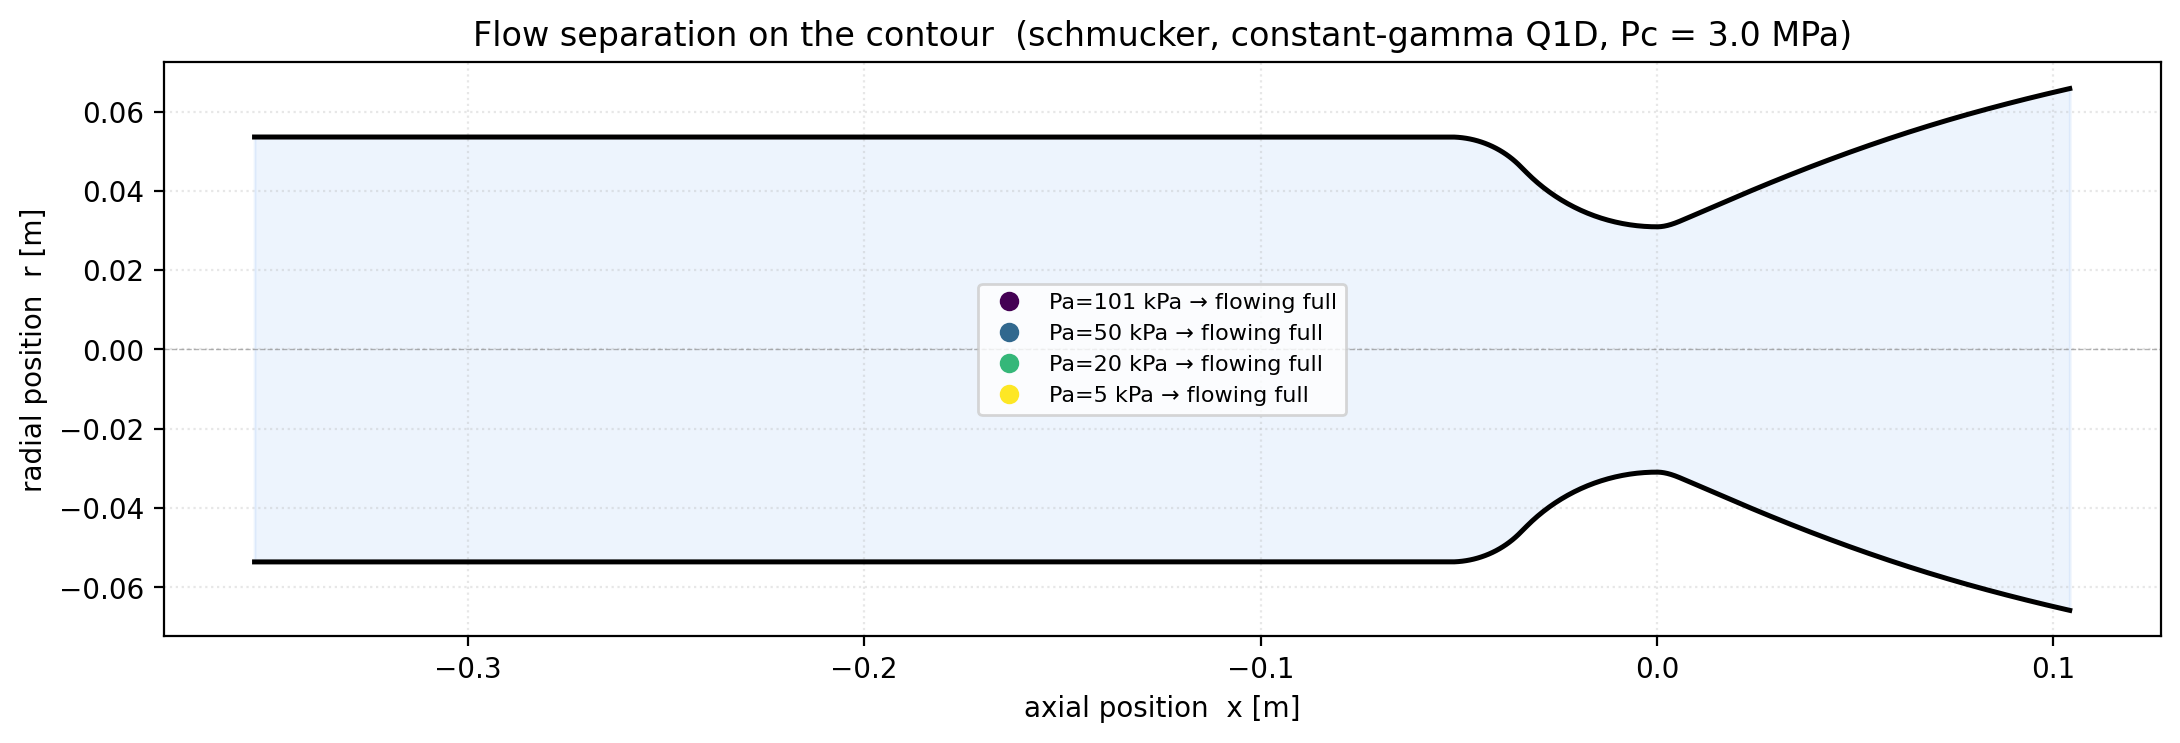
\includegraphics[width=0.5\linewidth,keepaspectratio]{figures/fresh/fresh_13kn_separation_check_contour.png}
\caption{Separation screen written by the fresh 13 kN run (separation\_contour.png): Schmucker criterion, constant-gamma Q1D, Pc = 3.0 MPa; flowing full at Pa = 101, 50, 20 and 5 kPa. This is an attached-flow FSS onset screen only.}
\label{fig:s04-separation}
\end{figure}

\lead{wall\_pressure.py and atmosphere.py}
\code{wall_pressure.py} computes $A(x)=\pi y(x)^2$ and inverts the area--Mach relation, on the subsonic branch up to the throat index and the supersonic branch after it. It then applies the isentropic pressure ratio and flags any $dp/dx>0$ downstream of the throat as a separation risk, ``per NASA SP-8120''. With a frozen expansion it uses the frozen stations and also returns $T(x)$ and $\gamma(x)$. The module imports \code{matplotlib.pyplot} at load time (:15). For that reason \code{raosim/benchmarks.py:537} carries its own copy of the calculation (``to avoid plotting imports'').

The \code{atmosphere.py} header claims a simplified ISA ``up to $\sim$86\,km'', using ``the standard 7-layer \ldots{} model for the first three key layers''. The code has three segments: 0--11\,km at $-6.5$\,K/km, 11--20\,km isothermal at 216.65\,K, and 20--47\,km at $+1.0$\,K/km. Above 47\,km it uses an isothermal 270.65\,K exponential tail, which its comment calls ``very rough''. A check run gives 228.65\,K and 868.0\,Pa at 32\,km. The job loader accepts only $[0, 32000]$\,m because ``beyond that it does not implement the next ISA lapse segment'' (\code{raosim/mdo/job.py:360-368}).

\subsection{Governing documents}

{\small
\begin{longtable}{@{}P{0.33\linewidth}P{0.12\linewidth}P{0.10\linewidth}P{0.37\linewidth}@{}}
\toprule
Document (new path) & Type & Status & Content for S04 \\
\midrule
\endhead
\code{docs/subsystems/S04-performance-and-off-design/FROZEN_VARIABLE_CP_EXPANSION.md} & subsystem basis & active & Frozen $C_F$/$c^*$ equations; the screens may use the profile only ``for diagnostics''. The only document in the S04 folder. \\
\code{docs/audits/DIFFERENTIABLE_MDO_PLAN_EVALUATION_2026-07-22.md} (A.2.1) & audit & historical record & The cross-labelled separation criteria and their same-day fix; cited from \code{separation.py:32}. \\
\code{docs/program/PHYSICS_FIDELITY_ROADMAP.md} (Section 3) & roadmap & active & Separation is ``structurally incomplete'' (FSS only); plan for FSS/RSS and side loads. \\
\code{docs/audits/INPUT_EXECUTION_INTEGRITY_2026-09-09.md} & remediation record & active & Altitude conversion limited to the declared 0--32\,km range. \\
\code{docs/audits/CONTRACT_INTEGRITY_REMEDIATION_2026-09-05.md} (W01) & remediation record & historical record & Maps the job altitude through \code{atmosphere.pressure}. \\
\bottomrule
\end{longtable}
}

\subsection{Verification}

{\small
\begin{longtable}{@{}P{0.29\linewidth}P{0.63\linewidth}@{}}
\toprule
Test & What it pins \\
\midrule
\endhead
\code{tests/test_gas_dynamics.py}, \code{tests/test_engine.py} & Worked example, $\gamma=1.4$, $\epsilon=10$: $M_e\approx3.9226$, $p_e/p_0\approx0.007306$, $\nu\approx64.75^\circ$, $C_{F,\text{vac}}\approx1.647$, $c^*\approx1355$\,m/s, $I_{sp}\approx228$\,s, $\dot m=P_cA_t/c^*$ (tolerances 0.1--3\,\%); a LOX/RP-1 smoke run. \\
\code{tests/test_v2_features.py} & Wall pressure and Mach monotone; each criterion pinned to its Östlund form ($10^{-12}$); the four criteria cluster within 0.25--0.55\,$P_a$ at $P_c/P_a=30$; vacuum never separates. \\
\code{tests/test_fidelity_scope_gates.py} & Separation results declare FSS-only scope and return \code{side_load_n=None} with a reason. \\
\code{tests/test_jax_thermal_design_opt.py::test_schmucker_parity} & NumPy--JAX Schmucker parity ($10^{-8}$) and a finite vacuum margin. \\
\code{tests/test_frozen_flow.py} & The constant-$c_p$ dispatch equals the legacy result; a mismatched $\overline{M}$ is rejected; the wall-pressure and separation adapters use the frozen profile and reject a stale $P_c$ or $\epsilon$. \\
\code{tests/test_requirements.py} & Sea level gives 101325\,Pa; vacuum gives $0<P_a\le1$\,Pa; 12\,km equals \code{atmosphere.pressure}. \\
\code{tests/test_design_v2.py}, \code{tests/test_plotting.py} & A target thrust loses to an explicit $R_t$, and sizing reports its Q1D closure basis (error $10^{-12}$); the separation plot marks detachment. \\
\bottomrule
\end{longtable}
}
No test checks \code{atmosphere.isa()} against reference ISA values. The only atmosphere test compares \code{requirements} with the module itself.

\subsection{Maturity, limitations and known defects}

\begin{enumerate}
\item \textbf{Performance is Q1D, calorically perfect and attached.} No separation loss enters thrust, and $R_t$ is sized from the Q1D $C_F$. The \emph{LREKit Consolidated Technical Review} of 7 October 2026 records the same limit for the MDO in its open-issue list (item~8: ``contour changes cannot move thrust'').
\item \textbf{The traditional run records no separation verdict.} \code{summary.json} has no separation field. The screen exists only as \code{separation_contour.png} (failures printed and skipped, :5081-5082), evaluated at four fixed ambients (101.325, 50, 20, 5\,kPa) rather than the design ambient. The gates \code{separation_margin} and \code{wall_pressure_monotonic} exist only on the \code{design_nozzle_v2} and legacy paths, and the former checks the raw separated flag, not \code{design_margin_ok} (\code{validation.py:280-291}). \code{physics.structural_screen} turns a separation exception into a margin of 0 and omits the frozen expansion.
\item \textbf{FSS onset only} (\code{screening_not_cfd_validated}): no shock structure, no RSS and no side loads. The registry entry \code{separation.empirical_onset} (\code{model_registry.py:597}) names only ``Kalt-Badal/Schmucker'' and cites \code{hagemann1998.pdf}, not the four Östlund (2002) criteria that are implemented.
\item \textbf{The design ambient is a ratio.} \code{--pa-over-p0} defaults to 0.01, so changing $P_c$ silently changes $P_a$, and the default run is not a sea-level design. S04 does not choose $\epsilon$. The shipped sea-level examples use $\epsilon=4.524$, below the new S05 chart floor of 5, so their Bézier runs now stop in S05.
\item \textbf{Silent numerical fallbacks.} \code{mach_from_area_ratio} returns its last iterate without a convergence flag. \code{wall_pressure_distribution} replaces a failed inversion with $M=1$ (:101-102).
\item \textbf{Atmosphere defects.} The 20--47\,km segment uses one $+1.0$\,K/km lapse rate, so the temperature jumps from 243.65 to 270.65\,K at 47\,km and density drops by 10\,\% across the step (check run of \code{isa}). The docstring overstates the model. \code{requirements._ambient_pressure} (\code{requirements.py:337-364}) accepts any altitude $\ge 0$, whereas jobs stop at 32\,km.
\item \textbf{Registry gaps.} \code{atmosphere.py}, the wall-pressure screen, the built-in propellant table and the $\eta_{c^*}/\eta_{C_F}$ convention have no \code{ModelProvenance} entry. \code{gas_dynamics.py} cites an unidentified ``provided Rao-nozzle formulation document''.
\end{enumerate}

\subsection{Developer notes}

\begin{itemize}
\item \textbf{The performance identity} lives in \code{engine.py}. \code{design.throat_radius_for_target_thrust} must apply the same $C_{F}\eta_{C_F}$ product, so that the sized thrust closes (the CLI test checks this to $2\times10^{-12}$). The summary fields are written at \code{run_nozzle.py:4999-5033} and updated by the spray block at :6161-6175.
\item \textbf{Isentropic relations} in \code{gas_dynamics.py} feed S05, S06, S07 and S12. Their JAX twin \code{raosim/jax/primitives.py} claims term-for-term parity (``1e-10 on closed forms''), so change both together. Run \code{tests/test_jax_primitives.py} and the MOC/Rao suites after any change.
\item \textbf{A separation criterion change} goes into \code{separation.py} and, in lock-step, \code{raosim/jax/thermal.py:121}; the tests are \code{test_v2_features.py} and \code{test_jax_thermal_design_opt.py}. Update the registry entry \code{separation.empirical_onset} too. To persist a verdict, call \code{check_separation} at the design ambient near \code{run_nozzle.py:5068}.
\item \textbf{Wall-pressure changes} must also reach the private copy in \code{benchmarks.py:537}, or the plot helper can move out of \code{wall_pressure.py} so the copy can be deleted. \textbf{Atmosphere changes} go into \code{atmosphere.py}; going above 32\,km means widening the job gate (\code{raosim/mdo/job.py:360-368}), giving \code{requirements._ambient_pressure} the same limit, and adding reference-value tests.
\end{itemize}
